%============================
%User Management
%============================
\subsection{User Management}
This module is responsible for reading data from the client's user database. It will do this by making use of passport.js. The module will log a user into the system, given the correct credentials. This system will provide an authorization interface to other modules, to see if user with a given userID has the needed privileges. This module will also give an interface to other modules, to retrieve the user's details, given the user's userID. 

\subsubsection{Scope}
The scope of the Project module is shown in the figure below:
	\begin{figure}[H]
	    	\centering
	    	\fbox{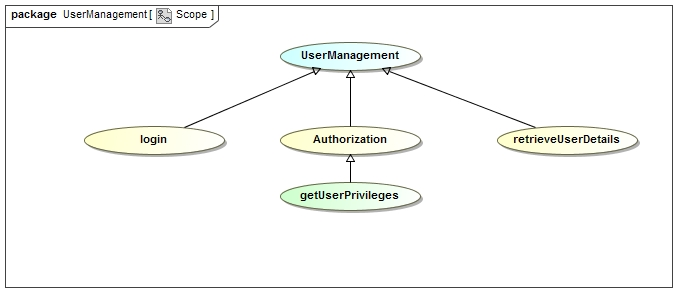
\includegraphics[width=1.0\textwidth]{UserManagementScope}}
	    	\caption{User Management Scope}
	    	\label{fig:UserManagementScope}
   	\end{figure}
\subsubsection{Use cases}

\paragraph{Login - priority: critical}
Takes user's credentials to log him into the system.

\begin{itemize}
	\item Services contract:\\ \\
	The loginRequest contains a user object. This user object in turn contains credentials that is sent sent to AuthenticateCredentials process that in turn authenticate the user with the username and password obtained from the credentials object. The login results contains a string that contains the user's id.
	\begin{figure}[H]
    	\centering
    	\fbox{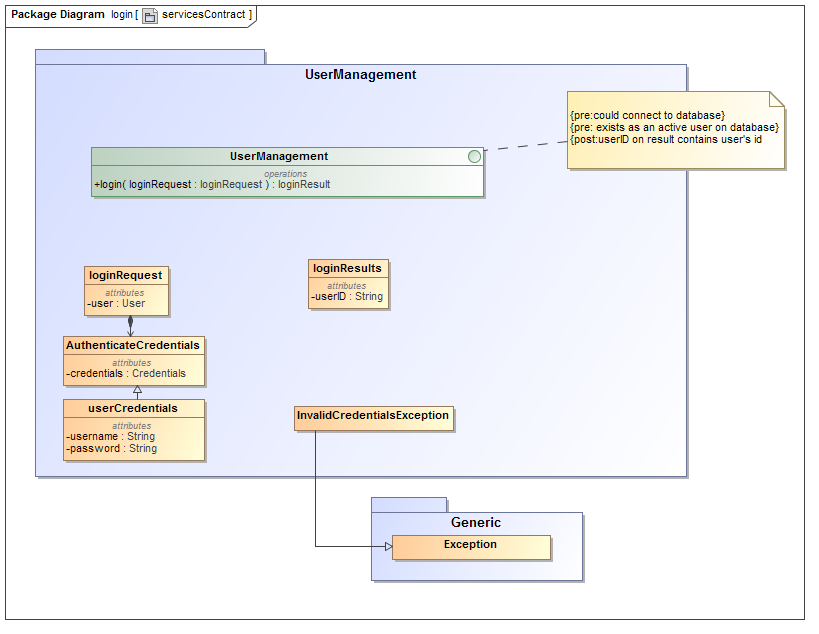
\includegraphics[width=1.0\textwidth]{servicesContractLogin}}
    	\caption{login services contract}
    	\label{fig:login_services_contract}
   	\end{figure}
\end{itemize}

\paragraph{Authorize - priority: critical}
Authorizes users with the right privileges to do what is requested.
\begin{itemize}
	\item Services contract:\\ \\
	The authorizationRequest contains only the user's id (the id alone, because user is already logged in) as a string. The authorizationResults contains the user's privileges.
	\begin{figure}[H]
    	\centering
    	\fbox{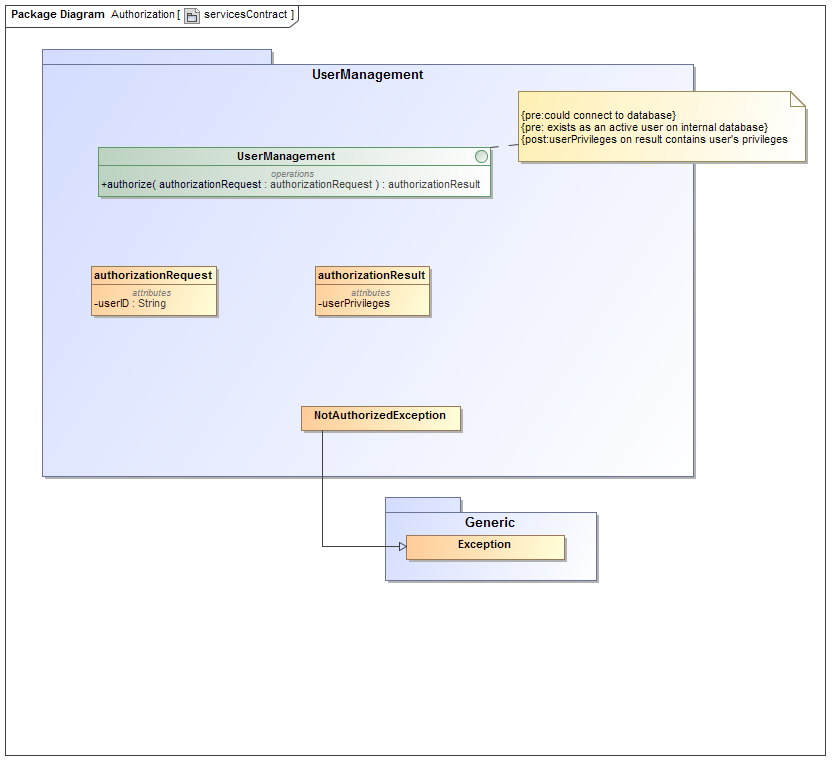
\includegraphics[width=1.0\textwidth]{servicesContractAuthorization}}
    	\caption{Authorization services contract}
    	\label{fig:Authorization_services_contract}
   	\end{figure}
\end{itemize}

\paragraph{retrieveUserDetails - priority: important}
This will get the details from the both the external and internal databases, to supply details to other modules in system as they need it.
\begin{itemize}
	\item Services contract:\\ \\
	The retrieveUserDetailsRequest contains the user's id as a string. The retriveUserDetailsResult contains the user's details which consists of a username, password, useremail, userPosition.
	\begin{figure}[H]
    	\centering
    	\fbox{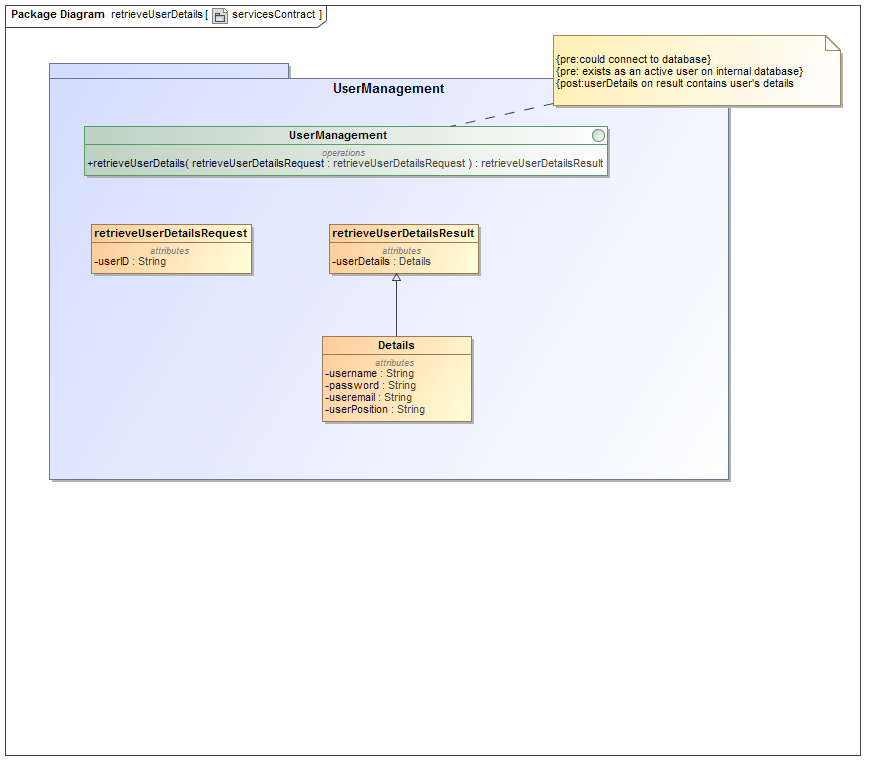
\includegraphics[width=1.0\textwidth]{servicesContractRetrieveUserDetails}}
    	\caption{RetrieveUserDetails services contract}
    	\label{fig:RetrieveUserDetails_services_contract}
   	\end{figure}
\end{itemize}

\paragraph{register - priority: important}
	Reigstrations of users are being handled by passport.js. This functionality is based on the strategy used for usermanagement, seeing as it will be unavailable if the LDAP strategy is used with passport.js.


\subsubsection{Domain model}
There is no domain model for this module, because it is purely an adapter that provides services to other modules in the system. The module does not persist information into the database.

%============================
%Project
%============================
\subsection{Project}
The project module is responsible for the representation and persistence of all projects that the system will use to do the estimations on. This module will allow for complex projects to be created, as well as to be updated. A project is represented as a tree, consisting of a top-level project node and lower-level task nodes.

\subsubsection{Scope}
The scope of the Project module is shown in the figure below
	\begin{figure}[H]
	    	\centering
	    	\fbox{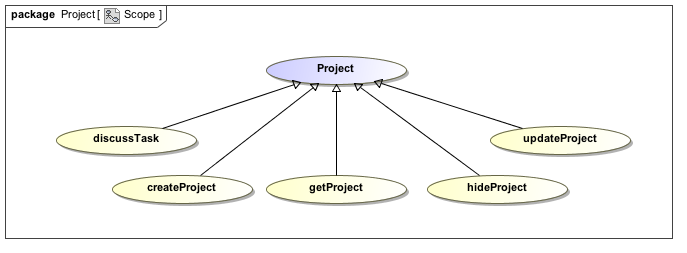
\includegraphics[width=1.0\textwidth]{projectScope}}
	    	\caption{Project Scope}
	    	\label{fig:Project_Scope}
   	\end{figure}
\subsubsection{Use cases}

\paragraph{Create a project - priority: critical}
Users with sufficient privileges can create projects. This will persist the project to the database.

\begin{itemize}
	\item Services contract:\\ \\
	The createProjectRequest contains the name of the project as well as the user who is creating the project. The function will allow the user to expand on the project in order to build a comprehensive project tree.
	\begin{figure}[H]
    	\centering
    	\fbox{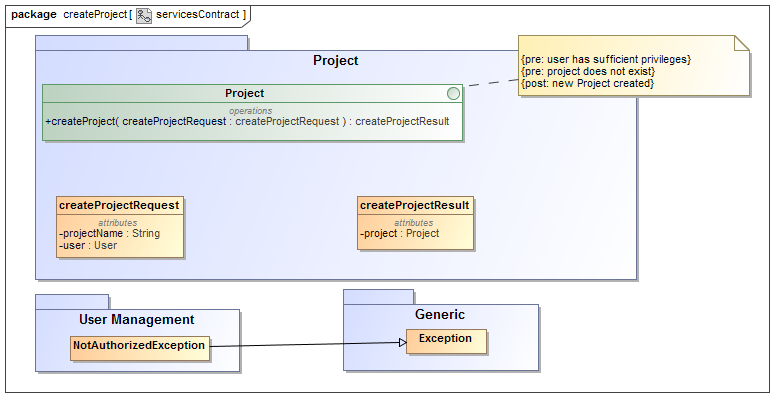
\includegraphics[width=1.0\textwidth]{servicesContractcreateProject}}
    	\caption{createProject services contract}
    	\label{fig:createProject_services_contract}
   	\end{figure}
\end{itemize}

\paragraph{Get project - priority: critical}
Users with sufficient privileges can retrieve projects to view them, or to be used for other purposes. This use case must thus return a representation of the project-tree, and not produce the output of the project tree.

\begin{itemize}
	\item Services contract:\\ \\
	The getProjectRequest contains the name of the Project that must be retrieved. The getProjectResult contains the Project that has been identified by the projectName.
	\begin{figure}[H]
    	\centering
    	\fbox{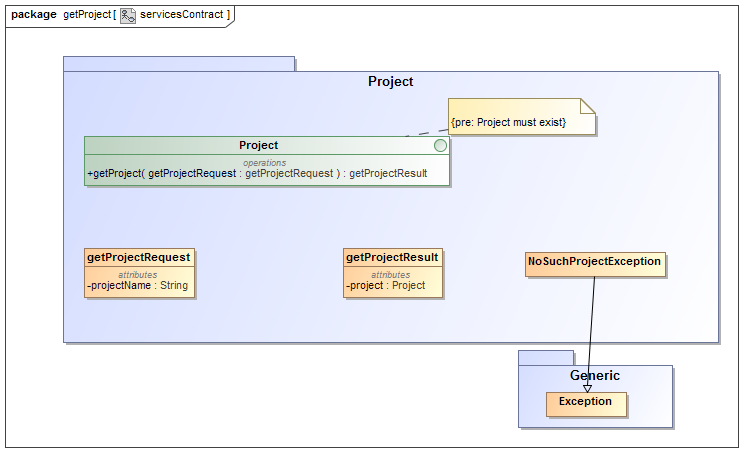
\includegraphics[width=1.0\textwidth]{servicesContractgetProject}}
    	\caption{getProject services contract}
    	\label{fig:getProject_services_contract}
   	\end{figure}
\end{itemize}

\paragraph{Delete project}
Projects can be removed from the database entirely by deleting them. This action can only be done by authorised user such as the owner of a project.

\begin{itemize}
	\item Services contract:\\ \\
	The deleteProjectRequest contains a reference to the Project that must be deleted, which can be obtained by calling the getProject function.
	\begin{figure}[H]
    	\centering
    	\fbox{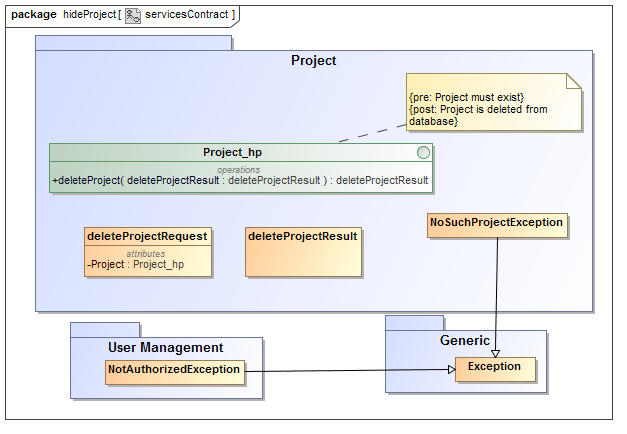
\includegraphics[width=1.0\textwidth]{servicesContractDeleteProject}}
    	\caption{deleteProject services contract}
    	\label{fig:deleteProject_services_contract}
   	\end{figure}
\end{itemize}


\paragraph{Update project - priority: critical}
This enables users to update projects, if they have sufficient privileges, by adding or removing task nodes to and from the project tree.

\begin{itemize}
	\item Services contract:\\ \\
	The updateProjectRequest contains a reference to the project that needs to be update which can be obtained by making use of the getProject functionality. The updateProjectRequest also contains a reference to the updated project, which can either be an entirely different project, or the same project as represented by oldProject, but with some changes applied to it.
	\begin{figure}[H]
    	\centering
    	\fbox{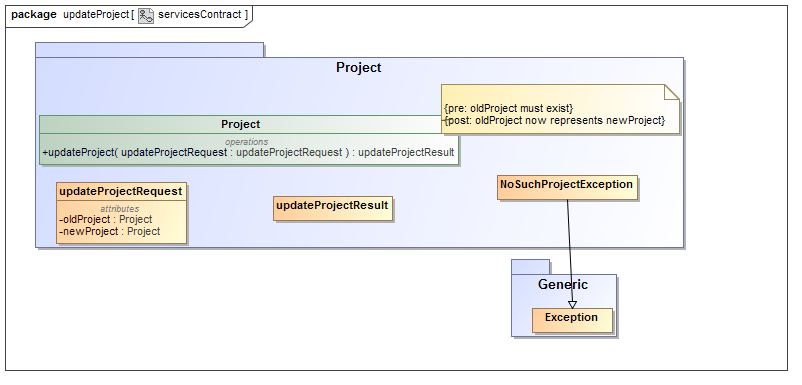
\includegraphics[width=1.0\textwidth]{servicesContractupdateProject}}
    	\caption{updateProject services contract}
    	\label{fig:updateProject_services_contract}
   	\end{figure}
\end{itemize}

\subsubsection{Domain model}
The domain model for the Project module requires that tasks being created and added to the tree, be persisted. Each project holds a reference to its parent, which is also of type Project. Furthermore, each Project holds a list of all its children, which once again, are also of type Project. Each instance of Project is represented as a Task object, which contains references to estimations made on that specific task.
\begin{figure}[H]
	\centering
	\fbox{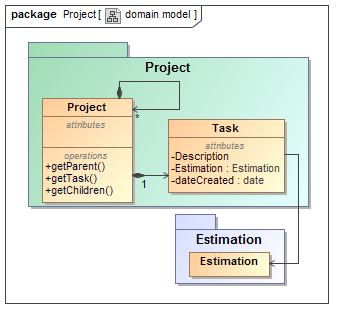
\includegraphics[width=0.5\textwidth]{projectdomainmodel}}
	\caption{Project domain model}
	\label{fig:Project_domain_model}
\end{figure}

%============================
%Estimation
%============================
\subsection{Estimation}
	The Estimation module will be responsible for handling all of the actions related to the estimation of a project. This involves allowing a user to place an estimate on a specific task as well as calculating the total estimation of a project.
\subsubsection{Scope}
	This is the estimation scope
	\begin{figure}[H]
	    	\centering
	    	\fbox{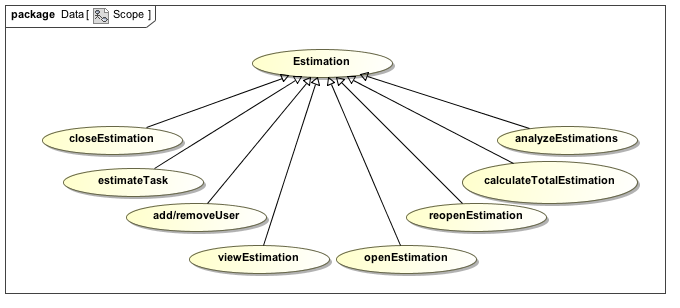
\includegraphics[width=0.6\textwidth]{Estimation_Scope}}
	    	\caption{Estimation Scope}
	    	\label{fig:Estimation_Scope}
   	\end{figure}
\subsubsection{Use cases}


	\paragraph{openEstimation- priority: critical}
	This enables users to publish projects for other users to estimate. The reason for this is to control when another user sees the project in his/her projects list and is able to estimate on the project.

	\begin{itemize}
		\item Services contract:\\ \\
		The OpenEstimationRequest will simply contain the userID of the person publishing the project as well as the projectID of the project being published. The openEstimationResult will contain minimal information, possibly only whether the publish was successfull.
		\begin{figure}[H]
	    	\centering
	    	\fbox{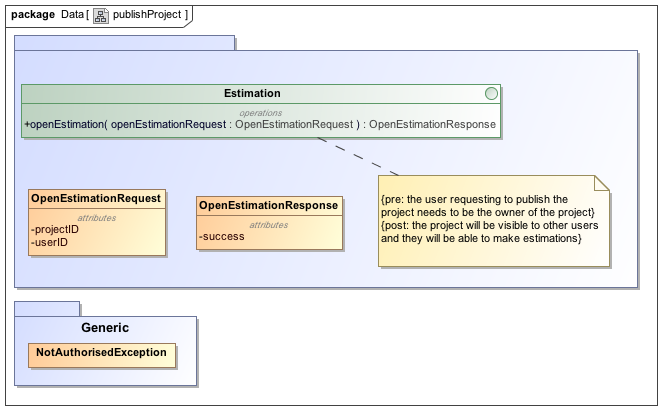
\includegraphics[width=1.0\textwidth]{publishProject}}
	    	\caption{openEstimation services contract}
	    	\label{fig:publishProject}
	   	\end{figure}

	\end{itemize}


	\paragraph{estimateTask - priority:critical}This system will allow a user to place an estimation on a task.
	\begin{figure}[H]
	    	\centering
	    	\fbox{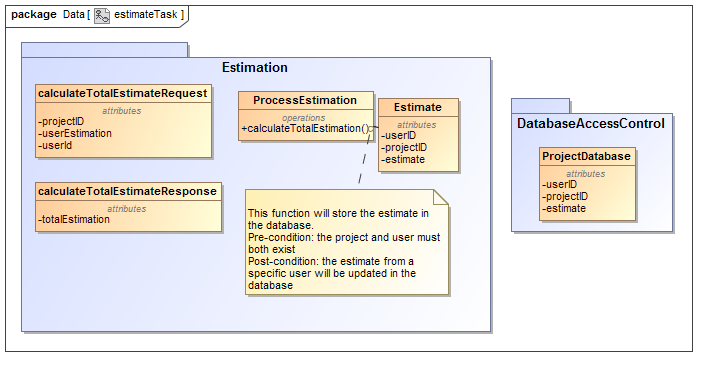
\includegraphics[width=0.9\textwidth]{Estimation_estimateTask}}
	    	\caption{Estimate Task}
	    	\label{fig:Estimation_estimateTask.png}
   	\end{figure}

	\paragraph{calculateTotalEstimation - priority:important}This system will traverse the project tree and calculate the total estimation of a project.
	\begin{figure}[H]
	    	\centering
	    	\fbox{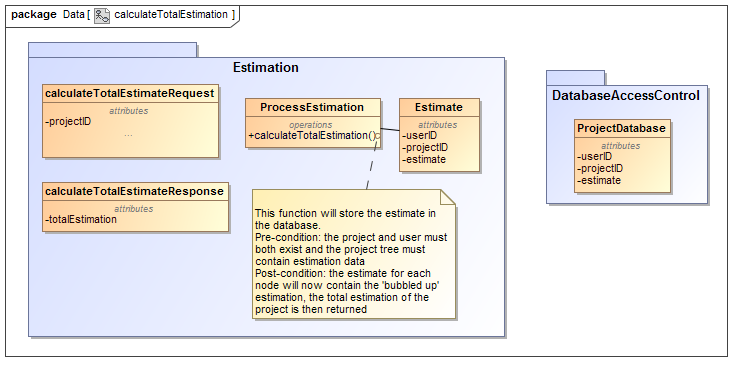
\includegraphics[width=0.9\textwidth]{Estimation_calculateTotalEstimation}}
	    	\caption{Calculate total estimation}
	    	\label{fig:Estimation_calculateTotalEstimation.png}
   	\end{figure}

	\paragraph{viewEstimation - priority:important}A user will be able to view his/her previous estimations for each project as a whole or for a specific node in the tree. Estimations made by other users will be hidden and only revealed when the project owner publishes the results. ViewEstimation will make use of the calculateTotalEstimation to calculate the estimation for a specific node in the project tree.
	\begin{figure}[H]
	    	\centering
	    	\fbox{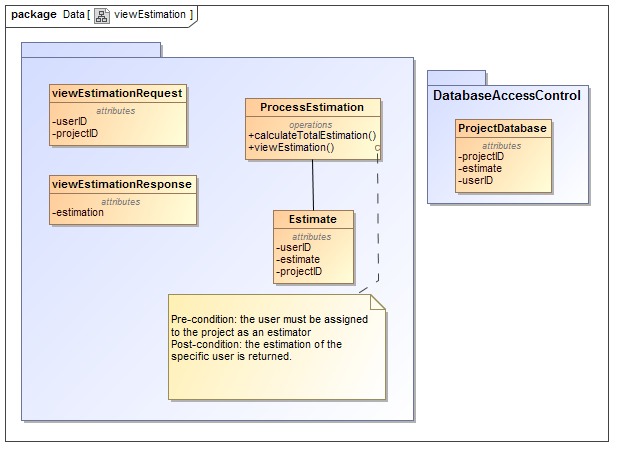
\includegraphics[width=0.9\textwidth]{Estimation_viewEstimation}}
	    	\caption{View estimation for user}
	    	\label{fig:Estimation_viewEstimation.png}
   	\end{figure}

	\paragraph{Add/Remove estimators - priority: important}
	Users with sufficient privileges can edit the estimators of a project. The changes to the estimators will then be propogated through the project tree and persisted to the database if the user chooses so.

	\begin{itemize}
		\item Services contract:\\ \\
		The user will be provided with a list of the current estimators as well as a list of possible estimators. The user will choose which estimators to add or remove.
		\begin{figure}[H]
	    	\centering
	    	\fbox{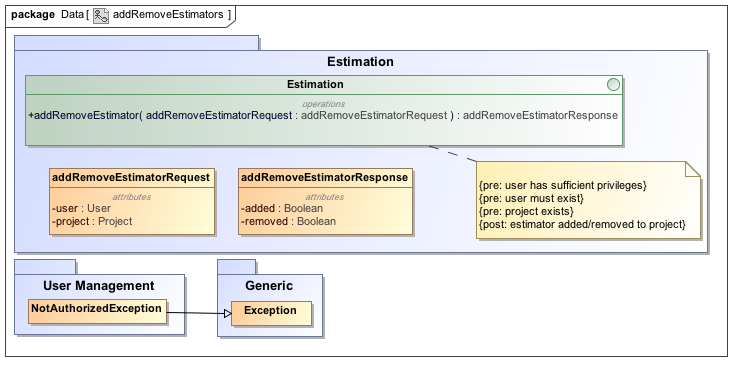
\includegraphics[width=1.0\textwidth]{servicesContractAddRemoveEstimator}}
	    	\caption{addRemoveEstimator services contract}
	    	\label{fig:addremove_estimators_services_contract}
	   	\end{figure}
	\end{itemize}


	\paragraph{reopenEstimation- priority: critical}
	This enables users to reopen projects for other users to estimate. The reason for this is to control when another user sees the project in his/her projects list and is able to estimate on the project for another round.

	\begin{itemize}
		\item Services contract:\\ \\
		The reopenEstimationRequest will simply contain the userID of the person publishing the project as well as the projectID of the project being published.
		
		\begin{figure}[H]
	    	\centering
	    	\fbox{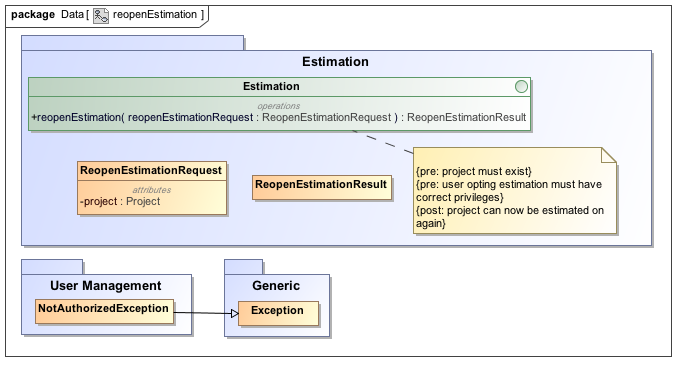
\includegraphics[width=1.0\textwidth]{servicesContractReopenEstimation}}
	    	\caption{reopenEstimation services contract}
	    	\label{fig:publishProject}
	   	\end{figure}
	\end{itemize}

	\paragraph{closeEstimation- priority: critical}
	Once all estimators have completed estimation, this function should fire automatically, so that no more further estimation can be done on the project until the owner decides to reopen estimation.

	\begin{itemize}
		\item Services contract:\\ \\
		The closeEstimationRequest contains the project that must be closed.
		\begin{figure}[H]
	    	\centering
	    	\fbox{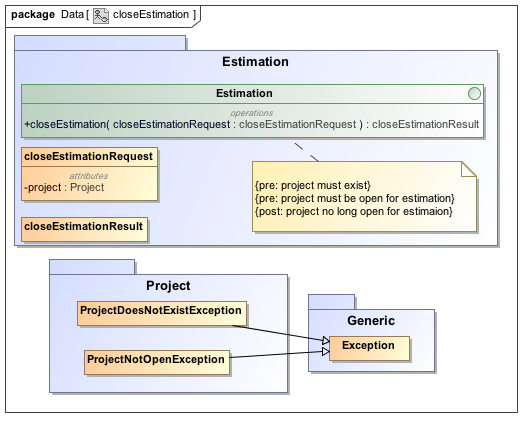
\includegraphics[width=1.0\textwidth]{servicesContractCloseEstimation}}
	    	\caption{closeEstimation services contract}
	    	\label{fig:closeEstimationServicesContract}
	   	\end{figure}

	\end{itemize}

	\paragraph{persistEstimation- priority: critical}
	This function will be called by closeEstimation, which then persists the estimation to the database.

	\begin{itemize}
		\item Services contract:\\ \\
		The persistEstimationRequest contains the project that must be closed.
		\begin{figure}[H]
	    	\centering
	    	\fbox{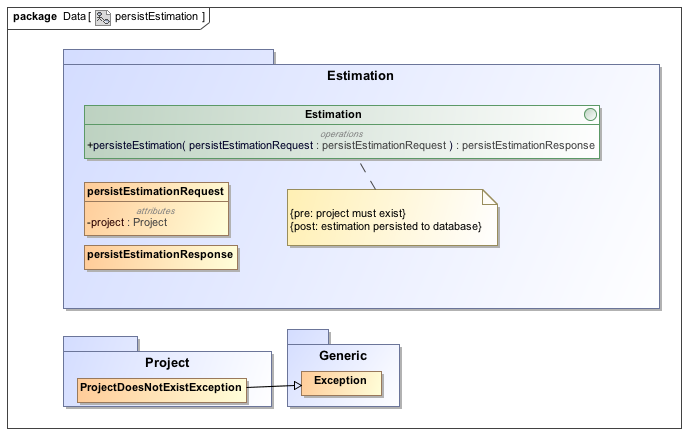
\includegraphics[width=1.0\textwidth]{servicesContractPersistEstimation}}
	    	\caption{persistEstimation services contract}
	    	\label{fig:persistEstimationServicesContract}
	   	\end{figure}

	\end{itemize}


\subsubsection{Domain model}
	\begin{figure}[H]
	    	\centering
	    	\fbox{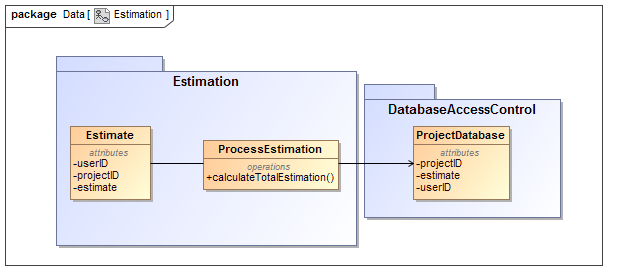
\includegraphics[width=0.9\textwidth]{Estimation_Domain}}
	    	\caption{Estimation Domain}
	    	\label{fig:Estimation_Domain.png}
   	\end{figure}
%============================
%Report
%============================
\subsection{Report}
The Report module will do statistical analysis on the data as well as draw graphs of the estimation data. This module will be responsible for any analysis of the data. It's functionality will be expanded as development continues. This module will retrieve all the data it requires from the database and then process that data to produce an appropriate result.
\subsubsection{Scope}
The scope of this module will be accessible to any user at this point in the development, the only authorization that will take place is the initial log in of the user.
	\begin{figure}[H]
	    	\centering
	    	\fbox{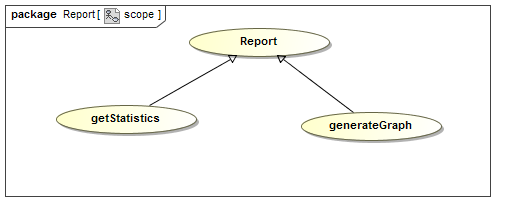
\includegraphics[width=0.8\textwidth]{Report_Scope}}
	    	\caption{Report Scope}
	    	\label{fig:Report_Scope.png}
   	\end{figure}
\subsubsection{Use cases}
	This section of the documentation will describe the use cases of the Report module.
	\paragraph{Statistical Analysis - priority:critical}
	User accessing this function will receive statistical analysis of the data for the chosen project.
	\begin{figure}[H]
	    	\centering
	    	\fbox{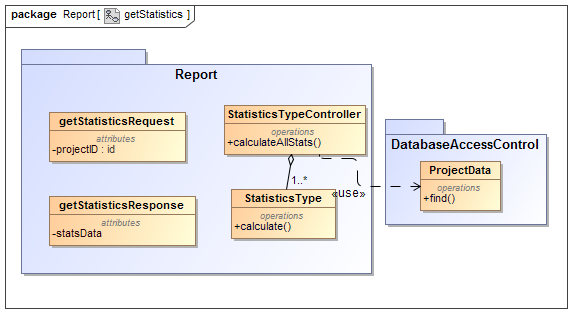
\includegraphics[width=0.8\textwidth]{Report_getStatistics}}
	    	\caption{Statistical Analysis Service Contract}
	    	\label{fig:Report_getStatistics.png Contract}
   	\end{figure}
	\paragraph{Generate Graphs - priority:critical}
	User accessing this function will receive a series of graphs of the data for the chosen project. 
	This will include for example a Bar Graph and Box Plot. The statistical data from the Delphi wide-band method 
	will be used as input to the graphs.
	\begin{figure}[H]
	    	\centering
	    	\fbox{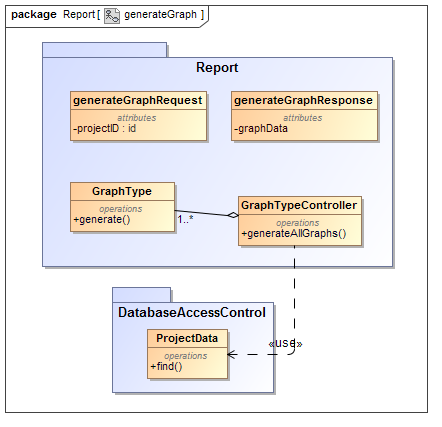
\includegraphics[width=0.8\textwidth]{Report_GraphGeneration}}
	    	\caption{Report Graph Generation Service Contract}
	    	\label{fig:Report_GraphGeneration.png Contract}
   	\end{figure}

\subsubsection{Domain model}
	\begin{figure}[H]
	    	\centering
	    	\fbox{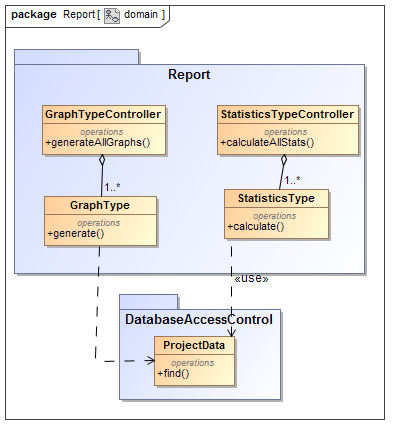
\includegraphics[width=0.9\textwidth]{Report_Domain}}
	    	\caption{Report Domain}
	    	\label{fig:Report_Domain.png}
   	\end{figure}
%============================
%Notification
%============================
\subsection{Notification}
This module will be responsible to notify all the users as required by the projects estimation. The estimation module will log a message request to the notification and add all the required users to notify.
\subsubsection{Scope}
This is the notification scope
	\begin{figure}[H]
	    	\centering
	    	\fbox{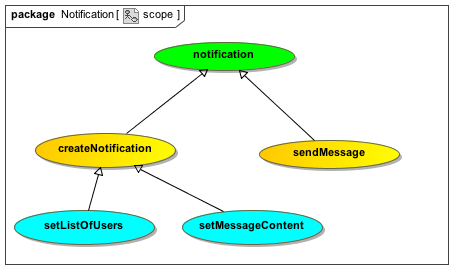
\includegraphics[width=0.8\textwidth]{Notification_Scope}}
	    	\caption{Notifications Scope}
	    	\label{fig:Notification_Scope}
   	\end{figure}
\subsubsection{Use cases}
The main purpose of notifications is to notify users with the required message. The estimation module will supply the list of users to notify and the contents of the message.
\paragraph{sendMesssage -- priority:niceToHave}
We will send the email to the destination address through the use of node mailer. 
\paragraph{createNotification -- priority:niceToHave}
The estimation module will create a notification request and send in to the notification module with the desired list of recipients.
	\begin{figure}[H]
	    	\centering
	    	\fbox{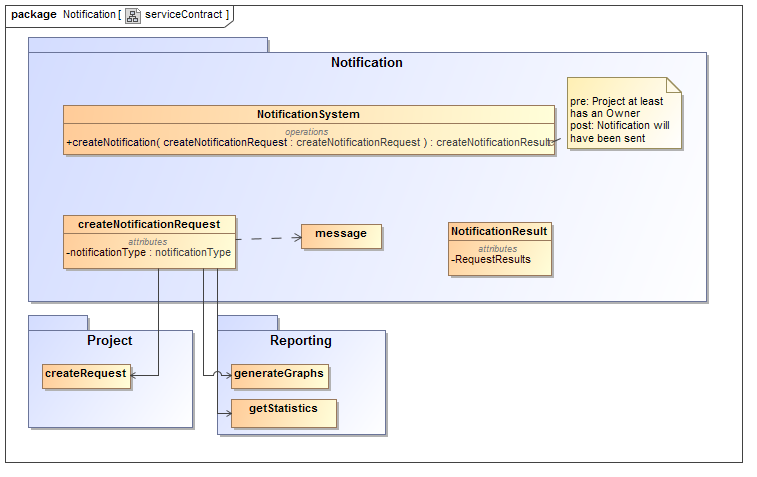
\includegraphics[width=0.8\textwidth]{NotificationServiceContract}}
	    	\caption{Notifications Service Contract}
	    	\label{fig:Notification_Service Contract}
   	\end{figure}
\subsubsection{Domain model}
	\begin{figure}[H]
	    	\centering
	    	\fbox{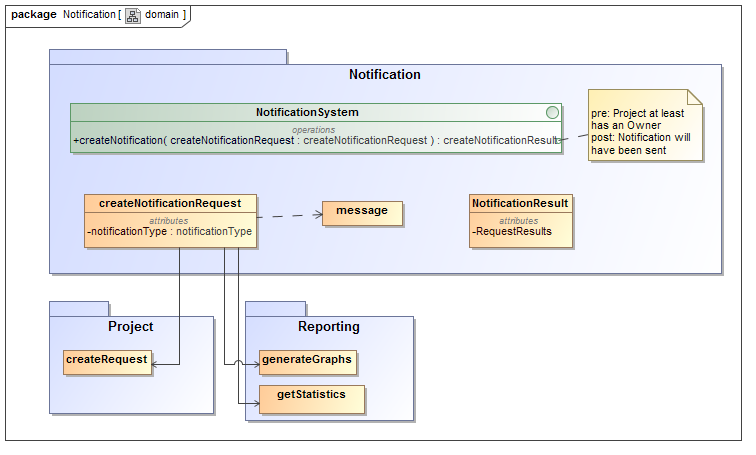
\includegraphics[width=0.8\textwidth]{NotificationDomain}}
	    	\caption{Domain Modelt}
	    	\label{fig:Domain Model}
   	\end{figure}
